\documentclass{article}
\usepackage[UTF8]{ctex}
% \usepackage[utf8]{inputenc}


\title{研究生选题报告 \\ 有机光电材料电荷传输过程的密度矩阵重整化群理论研究}
\author{李维唐}
\date{2019年6月}

\usepackage[numbers,sort&compress]{natbib}
\usepackage{graphicx}
\usepackage{subcaption}
\usepackage{geometry}
\usepackage{amsmath}
\usepackage{braket}

\graphicspath{{figures/}}

\geometry{a4paper,scale=0.8}

\newcommand{\He}{{\hat H}_{\text{e}}}
\newcommand{\Hph}{{\hat H}_{\text{ph}}}
\newcommand{\Heph}{{\hat H}_{\text{e-ph}}}
\DeclareMathOperator{\Tr}{Tr}

\begin{document}

\maketitle

\section{有机光电材料与电荷传输理论}

\subsection{有机光电材料简介}

有机光电材料可用于制备有机发光二极管(OLED)、有机太阳能电池(OPV或OSC)以及有机场效应晶体管(OFET)等器件,与传统的无机材料相比较,具有成本低、种类多、易加工、柔韧性好等优势,实际意义重大。

OLED器件(图~\ref{fig:intro-oled})可以将电能转化为光能,是最早问世的有机电子器件之一~\cite{TANG55,LO07,CHEN10}。OLED的发光机理可以以电子为例说明如下:
\begin{enumerate}
\item 电荷注入:在外电场作用下,电子从阴极注入到电子传输层;
\item 电荷传输:电子在电子传输层的LUMO上传输,并达到发光层;
\item 电荷复合:电子在发光层与从另一侧传输到发光层的空穴相遇,形成激子;
\item 发光:激子返回基态,放出光子。
\end{enumerate}

OLED可以用于制备柔性显示器件,在解决了电池等设备的柔性问题后,可以使人日常使用的电子设备弯曲、折叠,提升交互体验。现在正作为下一代显示器件进行大规模的工业化,折叠屏手机概念机如华为Mate X即将上市。

而OPV恰好是OLED的逆过程。人类目前赖以生存的化石燃料本质是动植物光合作用固定的太阳能,若能直接从太阳能高效地获得可以利用的能量,将为人类带来取之不尽的清洁能源(图~\ref{fig:intro-opv})。在科幻小说家和宇宙学家的想象中,发达的宇宙文明将建立包围他们的恒星的太阳能电池,称为戴森球~\cite{FREE60}。随着有机光电材料的迅猛发展,OPV的光电转化效率现已经超过$10\%$~\cite{YOU13,ZHAO16,CLARKE10,ALLEN11}。

\begin{figure}[ht]
  \centering%
  \subcaptionbox{有机发光二极管OLED
  \label{fig:intro-oled}}[6cm] 
    {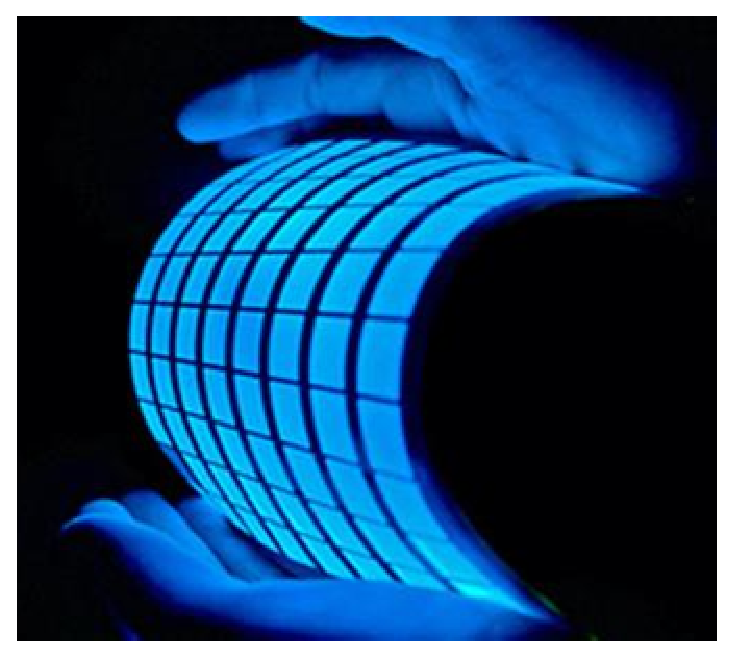
\includegraphics[height=4cm]{intro-oled}}%
  \hspace{2em}%
  \subcaptionbox{有机太阳能电池OPV
  \label{fig:intro-opv}}[6cm] 
      {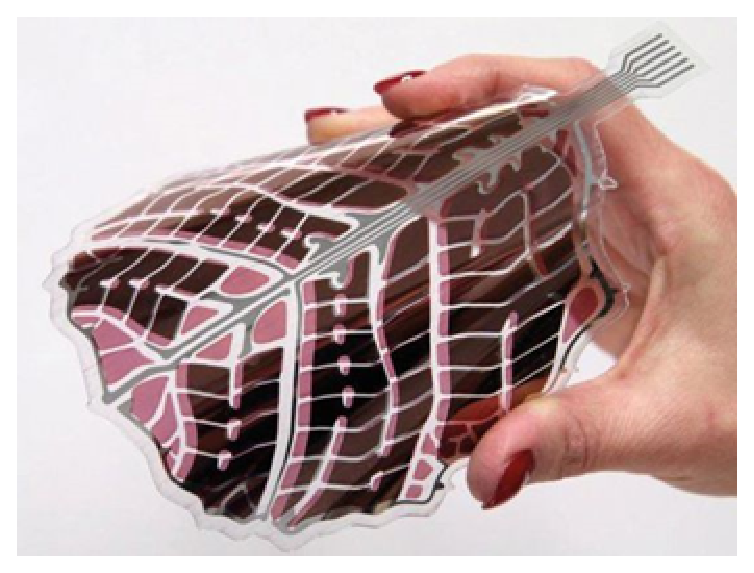
\includegraphics[height=4cm]{intro-opv}}
  \vspace{1em}
  \caption[有机发光二极管和有机太阳能电池示意图]{有机发光二极管和有机太阳能电池示意图(来自网络)}
  \label{fig:intro-intro}
\end{figure}

OFET是一类通过电场控制输出电流的半导体器件,这类器件是逻辑电路的基本组成部分~\cite{WEN11, WANG12,GELINCK10,MUCCINI06}。在OEFT中,电荷在源极注入,在漏极输出,两极之间有机半导体的性能,特别是电荷输运性能,对OFET器件的性能至关重要,目前,OFET的迁移率已经达到了约$10^2 \ \textrm{cm}^2/\textrm{Vs}$,与多晶硅持平~\cite{TSUT16}。

不论是OLED、OPV还是OFET,其中都涉及到电荷输运的过程。因此,为了促进有机光电材料的研究和应用,对有机材料中的电荷输运过程进行严格、精确的理论描述至关重要。

\subsection{有机小分子电荷输运性质的理论进展}

在有机半导体的电荷传输中,不仅要考虑电子的运动,还需要考虑原子核的运动。原子核的振动形成声子,而声子可以散射电子。这时,体系的哈密顿量可以分为电子、声子和电声耦合三个部分:
\begin{equation}
\label{eq:theory-mu-h}
\begin{aligned}
\hat H&= \He+ \Hph + \Heph \\
&=\sum_{mn}\varepsilon_{mn}a_m^\dag a_n+\sum_{\lambda}\hbar\omega_{\lambda}\left(b_{\lambda}^\dag b_{\lambda}+\frac{1}{2} \right ) + \sum_{mn\lambda}\hbar\omega_{\lambda}g_{\lambda mn}\left(b_{\lambda}^\dag + b_{\lambda} \right )a_m^\dag a_n
\end{aligned}
\end{equation}
其中$a_m^\dag(a_m)$是m格点上电子产生(湮灭)算符,其格点能为$\varepsilon_{mm}$;$b_{\lambda}^\dag(b_{\lambda})$是模式$\lambda$的声子产生(湮灭)算符,$\hbar\omega_{\lambda}$是声子能量;$\varepsilon_{mn}$是分子$m$和$n$之间的转移积分;$g_{\lambda mn}$表征了局域(当$m=n$时,Holstein模型)或者非局域(当$m\ne n$时,Peierls模型)电声耦合强度。

根据电子耦合和电声耦合之间的相对大小不同,电荷输运的理论描述工具不同。具体来说,分为以下三种情况~\cite{SHUAI12,SHUAI11}:
\begin{itemize}
    \item 当电子耦合远小于电声耦合,分子振动将电荷显著地定域化时,将电子耦合视为微扰,用跳跃模型描述电荷传输;
    \item 当两者相当时,用Holstein-Peierls极化子模型描述电荷传输;
    \item 当电子耦合远大于电声耦合时,将电声耦合视为微扰,用能带模型描述电荷传输。
\end{itemize}
其中,当两者相当时,理论分析的难度最大,对电荷传输过程进行难以比较精确的描述。

\subsubsection{跳跃模型}

跳跃模型认为,电荷是高度局域化在格点中的,格点之间的电荷转移过程可以用Marcus电荷转移速率来描述:
\begin{equation}
\label{eq:intro-mcs}
k_{if}=\frac{|V_{fi}|^2}{\hbar}\sqrt{\frac{\pi}{\lambda k_BT}}\exp\left[-\frac{\left(\Delta G+\lambda \right )^2}{4\lambda k_BT} \right ]
\end{equation}
其中$V_{fi}$是初末态之间的电子耦合(转移积分),$\lambda$是重整能,$\Delta G$是初末态之间的能量差。
电荷在分子间跳跃的过程被描述为扩散过程,迁移率由爱因斯坦关系式描述~\cite{SCHEIN79}:
\begin{equation}
\label{eq:hopping-einstein}
\mu=\frac{e_0D}{k_BT}
\end{equation}
其中$e_0$是元电荷,$D$是扩散系数。对于一个$n$维的系统,$D$被定义为均方位移$\langle r^2 \rangle$与时间$t$之比:
\begin{equation}
\label{eq:hopping-diffusion}
D=\frac{1}{2n}\lim_{t\rightarrow \infty }\frac{\langle r^2 \rangle}{t}
\end{equation}

1993年,B$\ddot{\rm a}$ssler首次将跳跃模型应用于无序材料。得益于其直观性和有效性,跳跃模型被化学家和材料学家广泛用于新型有机半导体材料的设计,并取得了成功~\cite{SHUAI14,SOKO11}。2009年,Nan等人在跳跃模型和Marcus公式的基础上,考虑了核隧穿效应,提出了全量子电荷转移速率公式~\cite{NAN09}。这一公式可以很好地描述电荷在跳跃机理下表现出的“能带般(band-like)”的行为。

\subsubsection{极化子模型}

极化子模型认为,电子在传输时对周围环境有极化作用,电子和它的周围环境作为整体参与输运,称为极化子(polaron)。当极化范围与晶格常数相当时,称为小极化子,反之称为大极化子。极化子模型是最一般化的电荷输运理论,它本身并不假设电子耦合或者电声耦合中有某一个占主导地位。

在不同的温度范围下,极化子的输运可以体现为不同的形式:在低温下,声子耦合弱,以能带形式输运;高温下,声子耦合强,以跳跃模式输运。1959年,Holstein提出了一维分子晶体中局域电声耦合下的小极化子模型,以描述能带-跳跃转换~\cite{HOLST59}。2007年,Wang等人首次利用极化子模型在DFT水平下考虑了所有的电声耦合项,对萘晶体进行了研究~\cite{WANG07, WANG08}。计算得到的能带-跳跃转换温度为153 K,与实验结果吻合。尽管如此,Wang等人得到的迁移率绝对值是实验值的大约10到1000倍,显示出在该参数区域内对电荷传输现象进行精确描述的挑战性。

\subsubsection{能带模型}
能带模型最初用于金属导体,在这些体系中,电子可以近似地认为不受原子核振动的影响,在晶体中以Bloch波的形式运动。一些堆积高度有序、分子间耦合很强的有机材料,如多并苯和红荧烯,能带宽度达几百meV,也具有可以用能带模型解释的载流子输运性质。能带模型下,迁移率可以表示为:
% 如果有ref
\begin{equation}
\mu=\frac{e\tau}{m^*}
\end{equation}
其中$e$是元电荷,$\tau$是电子-声子散射的弛豫时间,$m^*$是电子的有效质量。可以从能带的曲率求得。

载流子在运动过程中可能被声子散射,随着温度的升高,声子对电子的电子的散射增加,迁移率会降低,这是能带输运的典型现象。电子与声子的耦合可以用形变势理论描述,这一理论最初由Bardeen和Shockley在1950年提出,用于描述单晶硅等无机半导体~\cite{BARD50},后来被用于DNA链\cite{LADIK66}、碳纳米管~\cite{SA08}、石墨烯纳米带~\cite{LONG09}等的理论研究。

\subsubsection{数值模拟方法}
除了理论上的分析以外,大量较高精度的数值模拟方法也被用于对Holstein模型中电荷扩散动力学的的研究,
包括级联运动方程(Hierarchical Equations of Motion, HEOM)~\cite{Chen15}、基于Davydov拟设的含时变分法~\cite{Yang10}、
量子主方程~\cite{Wang10},表面跳跃(Surface Hopping, SH)~\cite{Wang15}、含时波包扩散(Time-Dependent Wavepacket Diffusion, TDWPD)~\cite{Jiang16}、
以及含时密度矩阵重整化群(Time Dependent Density Matrix Renormalization Group, TD-DMRG)方法\cite{Yao17}。


\section{含时密度矩阵重整化群方法}
\subsection{密度矩阵重整化群简介}
密度矩阵重整化群(Density Matrix Renormalization Group, DMRG)是由White在1992年提出的一种数值计算方法,特别适用于一维量子多体问题的研究~\cite{White92, White93}。2002年后,DMRG发展出了各种进行含时演化的算法~\cite{Caza02, Luo03, Vidal04, White04, Delay04, White05td, Haeg11, Haeg16, Garnet09}。这些方法应用于虚时演化中,使DMRG可以研究有限温问题~\cite{Vers04, Zwolak04, White05ft, Bart13}。现代DMRG方法一般由矩阵乘积态(Matrix Product States, MPS)和矩阵乘积算符(Matrix Product Operator, MPO)的语言来描述~\cite{Schol11}。

\subsubsection{矩阵乘积态}

在研究量子体系时,一个难以逾越的重大困难就是所谓的“指数墙”的问题。对于一个有$N$个自由度,每个自由度有两个状态的体系来说,体系总的可能状态数为$2^N$。
当$N=10$时,总状态数的大小为1024,体系的哈密顿量可以进行精确对角化,动力学行为可以精确得到。
而当$N=40$时,总状态数需要大约8 TB内存才能进行存储,更遑论存储哈密顿量以及对角化、研究动力学行为了。一般地,对于有$\sigma_1\sigma_2\cdots\sigma_N $共$N$个自由度的体系来说,其状态可以表示为:
\begin{equation}
        | \Psi \rangle  = \sum_{\{\sigma\}} C_{\sigma_1\sigma_2\cdots\sigma_N }  \ket{ \sigma_1\sigma_2\cdots\sigma_N } 
\end{equation}
而要表示这一状态$C_{\sigma_1\sigma_2\cdots\sigma_N }$,需要有$\prod_i |\sigma_i|$个变量。所需变量数随$N$是指数增长的。
这意味着,不做任何近似,在当前的计算条件下研究大(高自由度)体系是不可能的。

幸运的是,$C_{\sigma_1\sigma_2\cdots\sigma_N }$在大多数情况下是十分稀疏的,存在被压缩的空间。将它表示为多个小张量的乘积即矩阵乘积态MPS,是一种可行的压缩方式。形式上,MPS的定义为:
\begin{equation}
\label{eq:mps-mps}
\begin{aligned}
    | \Psi \rangle & = \sum_{\{\sigma\}} C_{\sigma_1\sigma_2\cdots\sigma_N }  \ket{ \sigma_1\sigma_2\cdots\sigma_N } \\ 
    & = \sum_{\{a\},\{\sigma\}}
     A^{\sigma_1}_{a_1} A^{\sigma_2}_{a_1a_2} \cdots
           A^{\sigma_N}_{a_{N-1}}  \ket{ \sigma_1\sigma_2\cdots\sigma_N }
\end{aligned}
\end{equation}
式子中,$A^{\sigma_i}_{a_{i-1}a_{i}}$为一系列矩阵,这些矩阵相乘可以得到$C_{\sigma_1\sigma_2\cdots\sigma_N }$,$a_i$是连接各个$A^{\sigma_i}_{a_{i-1}a_{i}}$的指标,其维数$|a_i|$记为$M$。MPS可以当做是波函数的一种拟设。

对于给定的物理体系,一个MPS所包含的信息多少完全由$a_i$的维数决定。$a_i$的维数越高,MPS所包含的信息越多。
显然,任意的$C_{\sigma_1\sigma_2\cdots\sigma_N }$总是可以不唯一地做这样的分解。尽管在一定条件下,比如体系处于基态时,这样的分解可以简单地构造,且$a_i$的维度甚至可以限制到1,对于一般的情况,进行精确的分解需要巨大的$a_i$,这时$\prod_{i} A^{\sigma_i}_{a_{i-1}a_{i}}$并不是比$C_{\sigma_1\sigma_2\cdots\sigma_N }$更好的表示。然而如果进行近似,限制$a_i$到比较小的维数,从而将$C_{\sigma_1\sigma_2\cdots\sigma_N }$嵌入到一个低维空间中,则可以有效降低内存占用,并使进一步的计算变得可能。当然,进行这样近似的前提是嵌入过程的误差是可控的。

由于对$C_{\sigma_1\sigma_2\cdots\sigma_N }$进行的分解具有一定的冗余自由度,可以对MPS的具体形式做出一定的限制,使MPS相关的算法在形式和实现上更简单。
例如,当Eq.~\ref{eq:mps-mps}中的$A^{\sigma_i}_{a_{i-1}a_{i}}$满足:
\begin{equation}
\label{eq:left-cano}
    \sum_{\sigma_i, a_{i-1}}A^{\sigma_i*}_{a_{i-1}a'_{i}} A^{\sigma_i}_{a_{i-1}a_{i}} = I_{a'_i, a_i}, i \neq N
\end{equation}
时,称这个MPS为左规整(left-canonical)的,其中$A^{\sigma_i*}_{a_{i-1}a_{i}}$表示$A^{\sigma_i}_{a_{i-1}a_{i}}$的共轭,$I_{a'_i, a_i}$为单位矩阵。类似地,假如$A^{\sigma_i}_{a_{i-1}a_{i}}$满足:
\begin{equation}
    \sum_{\sigma_i, a_{i}}A^{\sigma_i*}_{a'_{i-1}a_{i}} A^{\sigma_i}_{a_{i-1}a_{i}} = I_{a'_{i-1}, a_{i-1}}, i \neq 1
\end{equation}
时,称这个MPS为右规整(right-canonical)的。此时为了便于区分,可以将符号$A$替换为$B$,即
$$
\sum_{\{a\},\{\sigma\}}
     B^{\sigma_1}_{a_1} B^{\sigma_2}_{a_1a_2} \cdots
           B^{\sigma_N}_{a_{N-1}}  \ket{ \sigma_1\sigma_2\cdots\sigma_N }
$$
表示了一个右规整的MPS。更进一步地推广,如下形式的MPS:
\begin{equation}
\sum_{\{a\},\{\sigma\}}
     A^{\sigma_1}_{a_1} A^{\sigma_2}_{a_1a_2} \cdots A^{\sigma_{n-1}}_{a_{n-2}a_{n-1}}C^{\sigma_n}_{a_{n-1}a_n}
     B^{\sigma_{n+1}}_{a_n a_{n+1}} \cdots
           B^{\sigma_N}_{a_{N-1}}  \ket{ \sigma_1\sigma_2\cdots\sigma_N }
\end{equation}
表示了一个从第1到$n-1$个格点是左规整的,而从第$n+1$到$N$个格点是右规整的MPS。

体现规整化MPS优越性的一个最直接的例子是$\ket{\Psi}$的模即$\braket{\Psi|\Psi}$的计算:
\begin{equation}
\begin{aligned}
    \braket{\Psi|\Psi} = & \bra{ \sigma_N\cdots\sigma_1 }
    \sum_{\{a'\},\{\sigma'\}}  A^{\sigma'_N*}_{a'_{N-1}} \cdots
            A^{\sigma'_1*}_{a'_1}
           \sum_{\{a\},\{\sigma\}}
     A^{\sigma_1}_{a_1}  \cdots
           A^{\sigma_N}_{a_{N-1}}  \ket{ \sigma_1\cdots\sigma_N }    \\
           = & \sum_{\{a\}, \{a'\},\{\sigma\}} A^{\sigma_N*}_{a'_{N-1}} \cdots
            A^{\sigma_1*}_{a'_1} A^{\sigma_1}_{a_1}  \cdots
           A^{\sigma_N}_{a_{N-1}}
\end{aligned}
\end{equation}
若$\ket{\Psi}$是左规整的,即满足Eq.~\ref{eq:left-cano},那么:
\begin{equation}
\begin{aligned}
     \braket{\Psi|\Psi} = & \sum_{\{a\}, \{a'\},\{\sigma\}} A^{\sigma_N*}_{a'_{N-1}} \cdots
            A^{\sigma_1*}_{a'_1} A^{\sigma_1}_{a_1}  \cdots
           A^{\sigma_N}_{a_{N-1}} \\ 
           = & \sum_{\{a\}, \{a'\},\{\sigma\}} A^{\sigma_N*}_{a'_{N-1}} \cdots
            A^{\sigma_2*}_{a_1a'_2} A^{\sigma_2}_{a_1a_2}  \cdots
           A^{\sigma_N}_{a_{N-1}} \\
           = & \sum_{\sigma_N, a_{N-1}} A^{\sigma_N*}_{a_{N-1}}
           A^{\sigma_N}_{a_{N-1}}
\end{aligned}
\end{equation}
也就是说,MPS中最右侧矩阵的模即是$\ket{\Psi}$的模。

在小节~\ref{sssec: compress},我们将会说明任何MPS总是可以被规整化。

\subsubsection{矩阵乘积算符}
\label{sssec: mpo}
与矩阵乘积态类似,包括哈密顿量在内的算符$\hat{O}$也可以分解为多个矩阵的乘积:
\begin{equation}
\label{eq:mps-mpo}
    \hat{O} = \sum_{\{a\},\{\sigma\},\{\sigma'\}}
     W^{\sigma_1, \sigma'_1}_{a_1} W^{\sigma_2, \sigma'_2}_{a_1a_2} \cdots
                    W^{\sigma_N, \sigma'_N}_{a_{N-1}} 
                    \ket{\sigma_1\sigma_2\cdots\sigma_N}
                    \bra{\sigma'_1\sigma'_2 \cdots \sigma'_N}
\end{equation}
与MPS不同的是,采用一定的技巧,MPO在大多数情况下可以人为地在较小的$a_i$下构造。以只有最近邻相互作用的有限大小横场伊辛模型(transverse field Ising model)为例,其哈密顿量为:
\begin{equation}
    \hat H = J \sum_{i=1}^{N-1} S_z^{(i)} S_{z+1}^{(i)} + h \sum_{i=1}^N S_x^{(i)}
\end{equation}
其中$J$为耦合强度,$h$为磁场强度,$N$为格点数目, $S_z^{(i)}$和$S_x^{(i)}$为对应于第$i$个格点自由度的泡利矩阵。这一哈密顿量可以精确写作矩阵乘积的形式:
\begin{equation}
    \hat H = 
    \begin{bmatrix} 
     h S_x^{(1)} & J S_z^{(1)} & \hat I 
    \end{bmatrix}
    \left \{
    \prod_{i=2}^{N-1} 
    \begin{bmatrix} 
    \hat I       & 0           & 0 \\
     S_z^{(i)}   & 0          & 0 \\
     h S_x^{(i)} & J S_z^{(i)} & \hat I 
    \end{bmatrix}
    \right \}
    \begin{bmatrix} 
    \hat I       \\
     S_z^{(N)}    \\
     h S_x^{(N)} 
    \end{bmatrix}
\end{equation}
通过令$N=2$可以简单地对其正确性做验证。

显然,MPO的构造方式不是唯一的,但一般来说构造的矩阵乘积算符$M$越小越好,因为MPO的$M$越小,MPS算法的计算量就相应越小。对于存在长程相互作用的体系,最优的$M$至少与$N$呈线性关系。对于不存在长程相互作用的体系,最优的$M$一般与$N$无关,例如本例中$M=3$。这一特点表明MPS对于一维物理问题存在独特优势。

矩阵乘积算符和其它算符一样,最重要的用途是作用到某个态上,得到一个新的态:
\begin{equation}
\begin{aligned}
    \hat{O} \ket{\Psi} = 
       & \sum_{\{a\},\{\sigma\},\{\sigma'\}}
         W^{\sigma_1, \sigma'_1}_{a_1} W^{\sigma_2, \sigma'_2}_{a_1a_2} \cdots
                        W^{\sigma_N, \sigma'_N}_{a_{N-1}} 
                        \ket{\sigma_1\sigma_2\cdots\sigma_N}
                        \bra{\sigma'_1\sigma'_2 \cdots \sigma'_N} \\
        & \sum_{\{a'\},\{\sigma'\}}
     A^{\sigma'_1}_{a'_1} A^{\sigma'_2}_{a'_1a'_2} \cdots
           A^{\sigma'_N}_{a'_{N-1}}  \ket{ \sigma'_1\sigma'_2\cdots\sigma'_N } \\
      = & \sum_{\{a\},\{a'\}, \{\sigma\},\{\sigma'\}}
           A^{\sigma'_1}_{a'_1} W^{\sigma_1, \sigma'_1}_{a_1} 
           A^{\sigma'_2}_{a'_1a'_2} W^{\sigma_2, \sigma'_2}_{a_1a_2} \cdots
           A^{\sigma'_N}_{a'_{N-1}} W^{\sigma_N, \sigma'_N}_{a_{N-1}}
           \ket{ \sigma'_1\sigma'_2\cdots\sigma'_N } \\
\end{aligned}
\end{equation}
如果令:
\begin{equation}
    \sum_{\sigma'_i} A^{\sigma'_i}_{a'_{i-1}a'_{i}} W^{\sigma_i, \sigma'_i}_{a_{i-1}a_{i}}
    = A'^{\sigma_i}_{\{a, a'\}_{i-1}\{a, a'\}_{i}}
\end{equation}
那么$\hat{O} \ket{\Psi}$就可以重新表示成MPS的形式:
\begin{equation}
    \hat{O} \ket{\Psi} = \sum_{\{a, a'\},\{\sigma\}}
           A'^{\sigma_1}_{\{a, a'\}_1} A'^{\sigma_2}_{\{a, a'\}_1\{a, a'\}_2} \cdots
           A'^{\sigma_N}_{\{a, a'\}_{N-1}}  \ket{ \sigma_1\sigma_2\cdots\sigma_N } 
\end{equation}
此时$M$由$|a'_i|$增大到$|a_i|| a'_i|$,MPS的总参数数目扩大到原先的$|a_i|^2$倍。


\subsubsection{矩阵乘积态的压缩}
\label{sssec: compress}
% todo: 单个svd的解释。任佳骏师兄放在了附录中
在小节~\ref{sssec: mpo}中,我们介绍了当MPO作用到MPS后,MPS的参数数目会急剧上升。
如果MPS对这种现象束手无策,那么MPO和MPS的应用就会收到很大限制。
实际上,矩阵乘积态最重要的特点之一是可以进行高效的压缩。通过压缩可以在保持MPS所表示的态基本不变的前提下,降低$M$。
一般来说,将MPO作用后的MPS进行压缩,可以在比较精确的前提下将MPS的$M$压缩到MPO作用之前的水平。

最简单的压缩方法是利用奇异值分解(Singular Value Decomposition, SVD)进行压缩,相当于进行连续多次近似的施密特分解。设$\Psi_{ij}$由$\ket{i}_A$和$\ket{j}_B$进行叠加得到,对$\Psi_{ij}$进行精确的施密特分解,相当于通过基变换将$\psi_{ij}$对角化:
\begin{equation}
    \begin{aligned}
        \ket{\Psi} & = \sum_{ij} \psi_{ij} \ket{i}_A \ket{j}_B \\
        & = \sum_{ij} \sum_a U_{ia}S_{aa}V_{aj}^{\dag} \ket{i}_A \ket{j}_B \\
        & = \sum_a \left ( \sum_i U_{ia} \ket{i}_A \right ) S_{aa} \left ( \sum_j V_{aj}^{\dag} \ket{j}_B \right ) \\
        & = \sum_a S_{aa} \ket{ii}_A \ket{ii}_B
    \end{aligned}
\end{equation}
此时所有信息都被保持,如果求和时进行截断,仅对奇异值比较大的态求和,丢弃奇异值比较小的态,就可以对$\psi_{ij}$进行压缩。设截断到$r$,则$\ket{\tilde \Psi} \approx \ket{\Psi}$可以表示为:
\begin{equation}
    \ket{\tilde \Psi} = \sum_a^r S_{aa} \ket{ii}_A \ket{ii}_B
\end{equation}
在MPS中,可以从一侧开始对每个矩阵依次进行这样的分解,直至另一侧,则整个MPS中的$M$得到降低。
若这个过程是从左向右进行的,不难发现压缩后整个MPS变成了一个左规整MPS。

另一种进行压缩的方法是变分法,即利用变分原理求得$\ket{\tilde \Psi}$使得$||\ket{\tilde \Psi} - \ket{\Psi}||_2$最小化。

\subsection{密度矩阵重整化群的含时演化方法}
\label{ssec:dmrg-propagation}
量子态的含时演化满足含时薛定谔方程:
\begin{equation}
    i\frac{\partial \Psi}{\partial t} = \hat H \Psi.
\end{equation}
若哈密顿量不含时,则形式上波函数在任意时刻$t$的状态有解析解:
\begin{equation}
\label{eq:formal-schrodinger}
    \ket{\Psi(t)} = e^{-i\hat{H}t} \ket{\Psi(0)}
\end{equation}
其中$e^{-i\hat{H}t}$本质上是一个算符。假设$\ket{\Psi(0)}$可以被表示为MPS,而$e^{-i\hat{H}t}$可以表示为MPO,那么$\ket{\Psi(t)}$可以由MPO作用于MPS上得到。但是在实际情况下$e^{-i\hat{H}t}$很难直接表示成有限$M$的MPO,需要对其进行近似。对于只包含最近邻相互作用的体系,可以使用Suzuki-Trotter分解的方法进行比较精确的计算~\cite{Vidal04},而更复杂包括非最近邻相互作用的体系可以利用time-step targetting(TST)方法~\cite{White05td, Garnet17}、含时变分原理(Time Dependent Variational Principle, TDVP)~\cite{Manthe92, Wang181, WANG182, LUBICH16}、切比雪夫(Chebyshev)多项式方法~\cite{Holzner11, Halimeh15}和克雷洛夫(Krylov)空间方法~\cite{Scholl05}等计算。

TST方法将求解$\Psi(t)$的问题视为一个微分方程的初值演化问题(initial value problem, IVP)。原则上,如果$\Psi(t)$已知且$\Psi(t)$的导数可以求得,那么就可以通过类似泰勒展开的方式计算$\Psi(t+\tau), \tau \xrightarrow{} 0$。 据此,从已知的$t=0$时刻出发,不断计算下一个$t+\tau$时刻的波函数,经过足够多的步数就可以求得$\Psi(t)$。
4阶龙格-库塔(4th order Runge-Kutta, RK4)方法是最常见的IVP演化方法:
\begin{equation}
        \begin{aligned}
        | k_1 \rangle & = -i \hat{H}(t) | \Psi(t) \rangle  \nonumber \\
        | k_2 \rangle & = -i \hat{H}(t + \tau/2) 
            (| \Psi(t) \rangle + \frac{1}{2}
            \tau | k_1 \rangle) \nonumber \\
        | k_3 \rangle & = -i \hat{H}(t + \tau/2) 
            (| \Psi(t) \rangle + \frac{1}{2} 
            \tau | k_2 \rangle) \nonumber \\
        | k_4 \rangle & = -i \hat{H}(t + \tau) 
            (| \Psi(t) \rangle +
            \tau | k_3 \rangle) \nonumber \\
        | \Psi(t+\tau) \rangle & = | \Psi(t) \rangle + \frac{1}{6} \tau(| k_1 \rangle +
        2 | k_2 \rangle + 2| k_3 \rangle + | k_4 \rangle)  \label{eq:RK4}
    \end{aligned}
\end{equation}
RK4方法每一步演化的误差是$\mathcal{O}(\tau^5)$,最终的累积误差为$\mathcal{O}(\tau^4)$。

而TDVP方法的思路是利用变分原理求得MPS中每个矩阵的运动方程,然后分别对他们做演化。TDVP有许多变种,但其核心思想都是将$\ket{\Psi}$的导数$\hat H \ket{\Psi}$投影到切空间中:
\begin{equation}
    \frac{\partial \ket{\Psi}}{\partial t} = -i \hat P_{T_{\Psi}M_{\text{MPS}}} \hat H \ket{\Psi}
\end{equation}
其中$\hat P_{T_{\Psi}M_{\text{MPS}}}$为投影算符算符。经过投影,$\ket{\Psi}$将始终在MPS所定义的流形上运动。

不同的TDVP方案一般有不同的投影算符。比如对于最近出现的投影算符劈裂(Projector Splitting, PS)方法来说,投影算符具有如下的形式~\cite{Haeg16}:
\begin{equation}
\begin{aligned}
    \hat P_{T_{\Psi}M_{\text{MPS}}} = & \sum_{n=1}^N \sum_{\{a\},\{a'\}}
     B^{\sigma_1*}_{a'_1} B^{\sigma_1}_{a_1} \cdots B^{\sigma_{n-1}*}_{a'_{n-2}a_{n-1}} B^{\sigma_{n-1}}_{a_{n-2}a_{n-1}}
     A^{\sigma_{n+1}*}_{a_n a'_{n+1}} A^{\sigma_{n+1}}_{a_n a_{n+1}} \cdots A^{\sigma_N*}_{a'_{N-1}} A^{\sigma_N}_{a_{N-1}} \\
    &  \ket{ \sigma_1\cdots\sigma_{n-1}\sigma_{n+1}\cdots\sigma_N }
       \bra{ \sigma_1\cdots\sigma_{n-1}\sigma_{n+1}\cdots\sigma_N } \\
    & - \sum_{n=1}^{N-1} \sum_{\{a\},\{a'\}}
     B^{\sigma_1*}_{a'_1} B^{\sigma_1}_{a_1} \cdots B^{\sigma_{n}*}_{a'_{n-1}a_{n}} B^{\sigma_{n}}_{a_{n-1}a_{n}}
     A^{\sigma_{n+1}*}_{a'_n a'_{n+1}} A^{\sigma_{n+1}}_{a'_n a_{n+1}} \cdots A^{\sigma_N*}_{a'_{N-1}} A^{\sigma_N}_{a_{N-1}} \\
    &  \ket{ \sigma_1\cdots\sigma_N } \bra{ \sigma_1\cdots\sigma_N }
\end{aligned}
\end{equation}

\subsection{密度矩阵重整化群的有限温算法}

因为MPS表示的是纯态,最直观的进行有限温动力学计算的方式是对初始态做采样。但由于体系的自由度非常高,这么做对算力的要求很大。
另一种比较直观的方式是将有限温下的密度矩阵$\rho$直接当成一个算符表示为MPO,
并围绕这一事实重新用公式表述DMRG相关算法如含时演化算法~\cite{Vers04, Zwolak04}。
这样做尽管比较麻烦,但原则上是可行的,不足之处在于计算量还是比较大,具体原因后面会说明。
最后一种也是我们实际采用的方式是将有限温下的密度矩阵$\rho$(混合态)“纯化”成为一个纯态MPS~\cite{White05ft}。

任何一个密度矩阵$\rho$都可以在一个更大的希尔伯特空间下表示为一个纯态~\cite{nielsen00},自由度变为原来的两倍。
一般记真实的空间为$P$,辅助空间为$Q$,纯化后的密度矩阵(记为$\ket{\Psi}$)的一种表示方式是:
\begin{equation}
    \ket{\Psi} 
      = \sum_{\{a\},\{\sigma^P\}, \{\sigma^Q\}}
     A^{\sigma_1^P}_{a_1} A^{\sigma^Q_1}_{a_1a_2} \cdots
           A^{\sigma_N^P}_{a_{2N-2}a_{2N-1}} A^{\sigma_N^Q}_{a_{2N-1}}  \ket{ \sigma^P_1\sigma^Q_1 \cdots \sigma^P_N \sigma^Q_N}    
\end{equation}
而真实的密度矩阵可由对$Q$求偏迹得到:
\begin{equation}
    \rho = \Tr_Q \ket{\Psi} \bra{\Psi}
\end{equation}

如果将
$$
\sum_{a_i} A^{\sigma_i^P}_{a_{i-1}a_{i}} A^{\sigma_i^Q}_{a_{i}a_{i+1}}
$$
重新表示为
$$
A'^{\sigma_i^P, \sigma_i^Q}_{a_{i-1}, a_{i+1}}
$$
那么$\ket{\Psi}$可以写作:
\begin{equation}
\label{eq:mps-tf}
    \ket{\Psi} = 
    \sum_{\{a\},\{\sigma^P\},\{\sigma^Q\}}
     A'^{\sigma^P_1, \sigma^Q_1}_{a_2}  \cdots
                    A'^{\sigma^P_N, \sigma^Q_N}_{a_{2N-1}} 
    \ket{ \sigma^P_1\sigma^Q_1 \cdots \sigma^P_N \sigma^Q_N}
\end{equation}

式Eq.~\ref{eq:mps-tf}和Eq.~\ref{eq:mps-mpo}形式上有相似之处,但含义完全不同。
在Eq.~\ref{eq:mps-mpo}中,不论是$\sigma_i$还是$\sigma'_i$都代表了真实的物理空间,
而在Eq.~\ref{eq:mps-tf}中,$\sigma^P_i$和$\sigma^Q_i$分别代表了真实的物理空间和辅助空间。
当对纯化后的态进行操作如作用算符时,作用于物理空间自由度,仅当要从纯化后的态获取混合态时才会对操作辅助空间自由度,对其求迹。
这也是纯化方法相对于直接将$\rho$表示为密度矩阵形式上的主要区别。此外,不难发现如果纯化后的波函数$M=m$,那么对应的密度矩阵算符
$M=m^2$。也就是说,纯化方法获得的波函数$\ket{\Psi}$是比直接将$\rho$表示为密度算符更紧凑、计算量也更小的一种表示。
这是因为对归一化的$\ket{\Psi}$求偏迹后得到的密度矩阵自动满足密度矩阵所必需的迹为1、厄米性等性质,
而直接将$\rho$表示成为密度算符具有更多的冗余自由度。

一般情况下,进行有限温动力学模拟的第一步是获得热平衡密度矩阵$\rho = e^{-\beta \hat H}$
\footnote{这里简便起见,省略了配分函数$Z$,因为首先$Z$太大无法计算,其次最后在计算任何物理量时$Z$都会消去。},
其中$\beta=\frac{1}{k_B T}$,$k_B$为玻尔兹曼常数,$T$为温度。热平衡密度矩阵可以通过从无限温即$\beta=0$出发做虚时演化来计算。
无限温时,体系中任何一个态都具有相同的布居概率:
\begin{equation}
\begin{aligned}
    \ket{\Psi(0)} = &
    \sum_{\{\sigma^P\},\{\sigma^Q\}}
    \ket{ \sigma^P_1\sigma^Q_1 \cdots \sigma^P_N \sigma^Q_N}       \\
    \rho(0) = & \Tr_Q \ket{\Psi(0)} \bra{\Psi(0)} = I
\end{aligned}
\end{equation}

则热平衡密度矩阵可以表示为:
\begin{equation}
\label{eq:imag-propagation}
\begin{aligned}
    e^{-\beta \hat H} = & e^{-\beta \hat H} I = e^{-\beta \hat H} \Tr_Q \ket{\Psi(0)} \bra{\Psi(0)} \\
    = & \Tr_Q \ket{e^{-\beta \hat H} \Psi(0)} \bra{\Psi(0)}  \\
    = & \Tr_Q \ket{e^{-\frac{\beta \hat H}{2}} \Psi(0)} \bra{\Psi(0)e^{-\frac{\beta \hat H}{2}}} \\
    = & \Tr_Q \ket{\Psi(\frac{\beta}{2})} \bra{\Psi(\frac{\beta}{2})}
\end{aligned}
\end{equation}
其中$\ket{\Psi(\frac{\beta}{2})} = \ket{e^{-\frac{\beta \hat H}{2}} \Psi(0)}$形式上和Eq.~\ref{eq:formal-schrodinger}类似,
只需令$t=\beta / i$即可利用小节~\ref{ssec:dmrg-propagation}中介绍的含时演化方法计算。

密度矩阵的动力学行为满足量子刘维尔方程:
\begin{equation}
    \frac{\partial \rho}{\partial t} = -i[\hat H, \rho].
\end{equation}
若哈密顿量不含时,则形式上$\rho$在任意时刻$t$的状态有解析解:
\begin{equation}
    \rho(t) = e^{-i \hat H t} \rho(0) e^{i \hat H t}
\end{equation}

假设初态是热平衡密度矩阵:
\begin{equation}
    \rho(0) = e^{- \beta \hat H} = \Tr_Q \ket{\Psi(\frac{\beta}{2})} \bra{\Psi(\frac{\beta}{2})}
\end{equation}
不难发现$\rho(t)$具有和Eq.~\ref{eq:imag-propagation}相同的形式:
\begin{equation}
\begin{aligned}
    \rho(t) = & e^{-i \hat H t} \rho(0) e^{i \hat H t} \\
            = & e^{-i \hat H t} \Tr_Q \ket{\Psi(\frac{\beta}{2})} \bra{\Psi(\frac{\beta}{2})} e^{i \hat H t} \\
            = & \Tr_Q \ket{e^{-i \hat H t} \Psi(\frac{\beta}{2})} \bra{\Psi(\frac{\beta}{2}) e^{-i \hat H t}}
\end{aligned}
\end{equation}
$\ket{e^{-i \hat H t} \Psi(\frac{\beta}{2})}$即可利用小节~\ref{ssec:dmrg-propagation}中介绍的含时演化方法计算。

\section{计划研究的科学问题}
\subsection{电荷传输过程中的同位素效应}
\subsubsection{研究背景}
同位素取代是研究核的运动对有机半导体中电荷传输动力学影响的一种有效方式。同位素效应指(重)同位素取代前后电荷传输速率的相对变化。
Munn等人首先在1970年研究了Holstein模型下的同位素效应~\cite{Munn70}。他们发现在“相干慢电子”极限下同位素效应是负数,其他情况下是正数。
他们随后对氘代蒽的同位素效应进行了实验测试,发现该体系有75\%概率存在正的同位素效应~\cite{Munn70exp}。1971年,Morel等人报道蒽经过氘代后迁移率提升了至少2.5倍~\cite{Morel71}。这一离奇的结果被他们1973年的实验所推翻,他们得出结论在c方向氘代蒽的同位素效应大约是负10\%~\cite{Morel73}。除此之外,萘和红荧烯体系分别被发现几乎没有同位素效应~\cite{SCHEIN79, Xie13}。而实验测得导电高分子具有负的同位素效应~\cite{Shao14}。

我们课题组曾经基于核隧穿电荷转移理论预测在跳跃极限下同位素效应应为负值~\cite{NAN09, Jiang14, Jiang15, Jiang18}。
最近Frisbie等人开展的对同位素取代红荧烯体系的实验也与我们的预测相符~\cite{Ren17}。
然而,Frisbie等人对这一现象的解释却是基于涨落无序限制的电荷扩散理论~\cite{Fratini16, Troisi06}和有效带宽收窄效应~\cite{Hann041}。

电荷传输的同位素效应之所以一直存在争议,是因为这是一个不论在实验上还是理论上都有很大挑战性的问题。
实验上,合成高纯度的氘代分子进行精确的迁移率测试成本高、难度大。
理论上,电荷传输理论往往过于粗糙或者只适用于特定极限,难以对相对数值不大的同位素效应进行精确描述。

基于此我们计划使用数值上几乎精确的TD-DMRG方法,研究电荷传输中的同位素效应问题。这一方法相较于其他的研究电荷传输的理论有如下几个优点:
\begin{itemize}
    \item 包括电子和振动在内的自由度都进行量子力学处理,捕捉核的量子效应;
    \item 在模型哈密顿量下可以得到几乎精确的动力学结果;
    \item 可研究的参数空间既包括跳跃模型和能带模型适用的区域,也包括很难处理的转移积分和重整能相近的中间区域。
\end{itemize}

当然,使用更好的方法,往往意味着需要更大的计算量。受算力限制,TD-DMRG目前最多只能在一定体系下处理数千个自由度,相当于数十到两三百个分子。

\subsubsection{初步结果}
作为初步探索,我们基于一个简单的均质Holstein模型开展研究。模型中,每个分子只有一个振动模式,各个分子完全等同,形成一个一维链,哈密顿量为:
\begin{eqnarray}
	\label{eq:hamil}
	\hat H && =	\He + \Hph + \Heph,  \\
	\label{eq:he}
	\He && = \sum_{i} \left(a_i^\dagger a_{i+1} + \text{h.c.}\right),  \\
	\label{eq:hph}
	\Hph && = \sum_{i} \frac{\omega}{J} b_{i}^\dagger b_{i}, \\
	\label{eq:heph}
	\Heph && = \sum_{i} \frac{g\omega}{J} a_i^\dagger a_i
	(b_{i}^\dagger + b_{i})
\end{eqnarray}
其中$J$为转移积分。利用$J$将声子的振动频率约化,体系只留下了两个自由度$\frac{\omega}{J}$和$g$。
我们将这两个自由度组合得到约化频率$\frac{\omega}{J}$和约化重整能$\frac{\lambda}{J} = \frac{g^2 \omega}{J}$作为系统的两个自由参数。
因为这两个参数在电荷传输研究中被广泛使用~\cite{SHUAI12}。通过调节这两个参数,同时计算在演化时间$t=6$时电荷扩散的均方位移(Mean Square Displacement, MSD):
$$
\text{MSD}(t) = \braket{\Psi(t)|\hat {r}^2|\Psi(t)} - \braket{\Psi(t)|\hat r|\Psi(t)} ^ 2
$$
就可以比较不同参数范围内电荷的扩散速度,结果如图~\ref{fig:msd}所示:
\begin{figure}[ht]
    \centering
	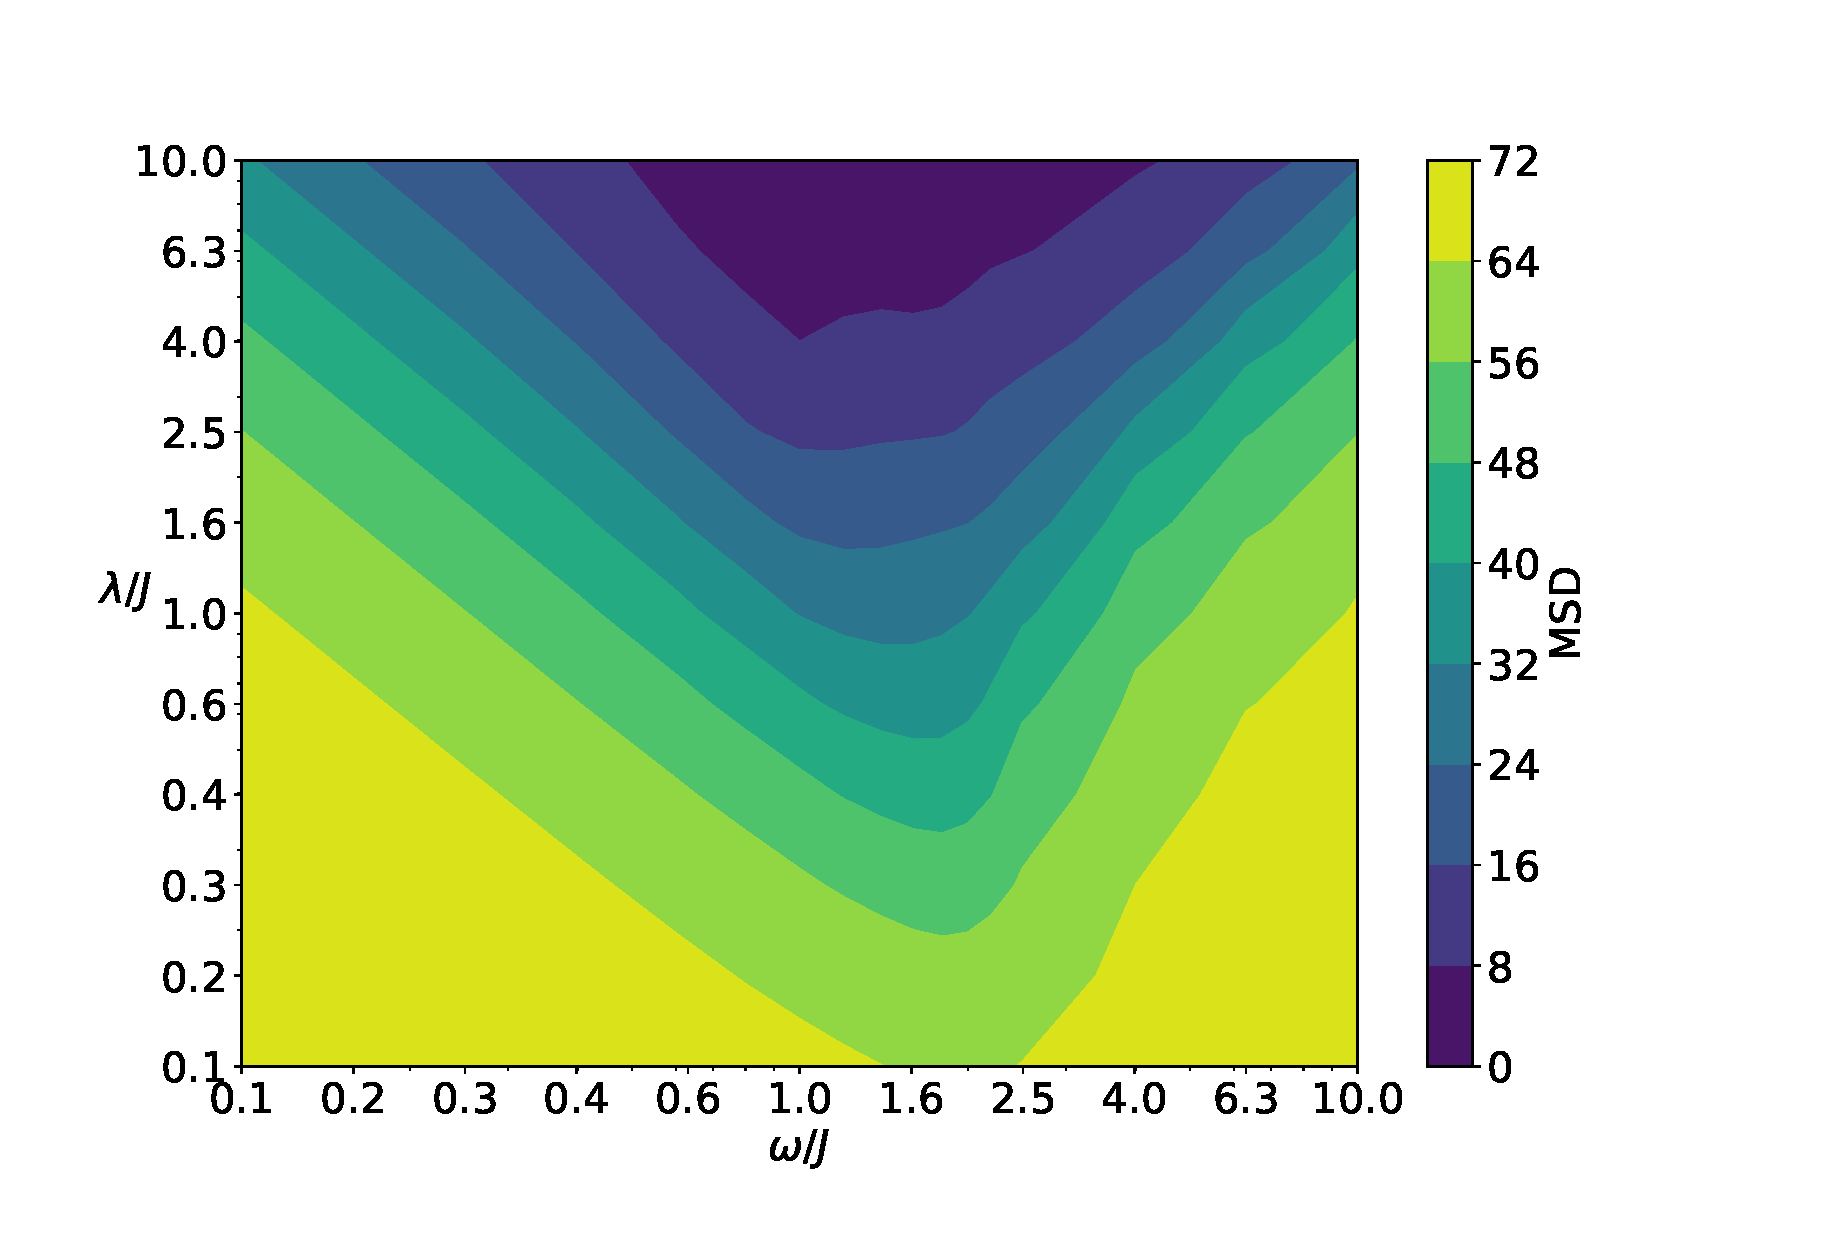
\includegraphics[width=.6\linewidth]{msd}
	\caption{\label{fig:msd}不同$\frac{\omega}{J}$和$\frac{\lambda}{J}$下$t=6$时刻的MSD。两个轴都是对数坐标。}
\end{figure}

从图中可以看出,相同约化频率下,重整能越大,电荷的迁移速度越慢,这和电荷输运过程的一般常识是一致的。但在相同的约化重整能下,MSD随约化频率的变化并不是单调的。
在有机半导体的电荷输运问题中,一般认为IE是由相同的重整能下声子振动频率的变化导致的~\cite{Ren17, Jiang15, Shao14},因此依照下式即可计算IE:
\begin{equation}
    \newcommand{\MSDa}{\text{MSD}_{\frac{\lambda}{J}, \frac{\omega_1}{J}}}
    \newcommand{\MSDb}{\text{MSD}_{\frac{\lambda}{J}, \frac{\omega_2}{J}}}
    \text{IE} = \frac{ \MSDa- \MSDb}{\MSDa} \bigg / \frac{\omega_1- \omega_2}{\omega_1}  \delta \omega
\end{equation}
其中$\text{MSD}_{\frac{\lambda}{J}, \frac{\omega}{J}}$代表在$\frac{\lambda}{J}$和$\frac{\omega}{J}$参数下$t=6$时刻的MSD, 
$\delta \omega$代表同位素取代后$\omega$的减小幅度。这个式子进行了线性插值的近似,但对最后定性结果没有影响。
这里我们根据文献报道~\cite{Ren17, Jiang15},取$\delta \omega = 3\%$。计算得到的IE如图~\ref{fig:ie}示。

\begin{figure}[ht]
    \centering
	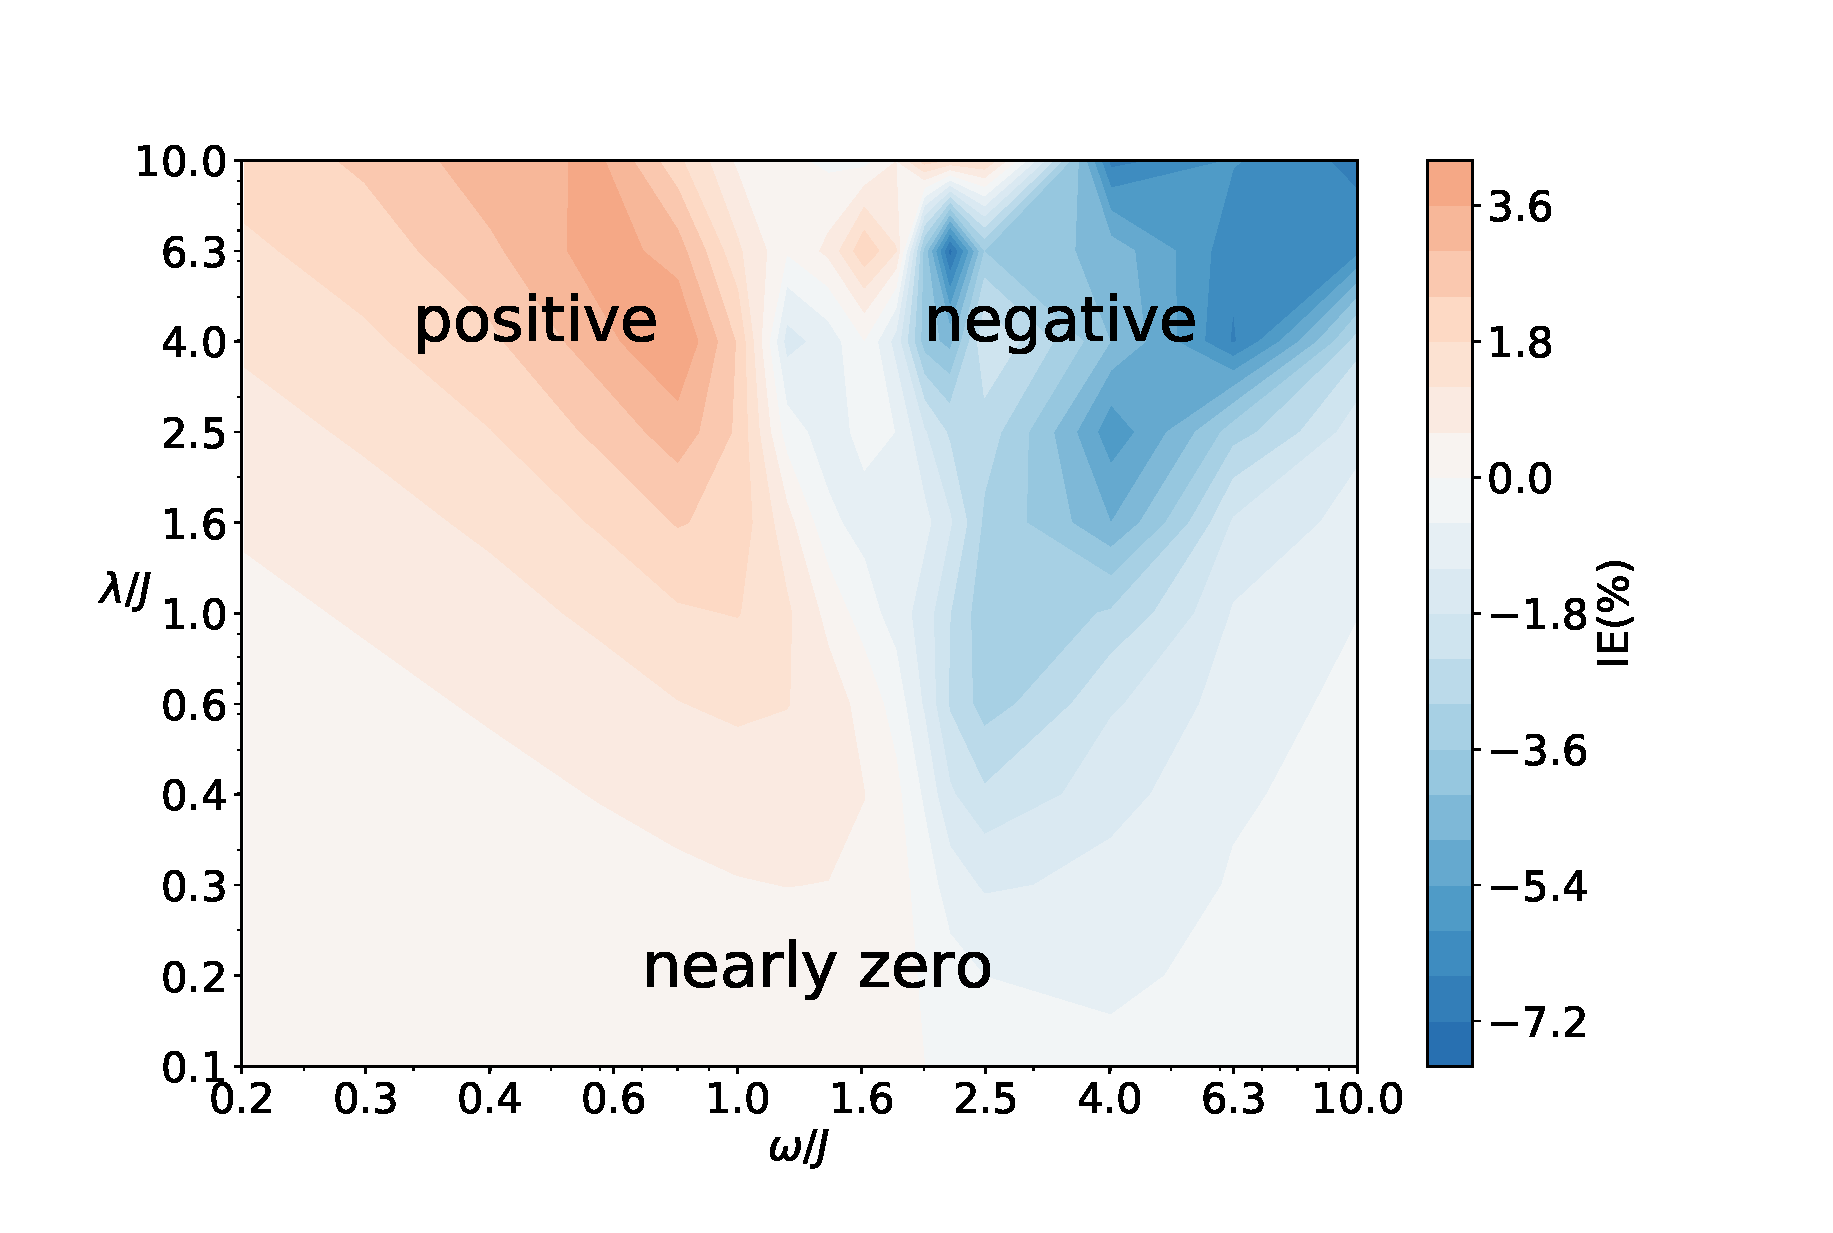
\includegraphics[width=.6\linewidth]{ie}
	\caption{\label{fig:ie}在全参数空间下的同位素效应。蓝色、白色和红色区域分别代表负、零以及正同位素效应。两个轴都是对数坐标。}
\end{figure}

图~\ref{fig:ie}实际上是图~\ref{fig:msd}沿$\frac{\omega}{J}$方向的导数。从图中可以看出,当重整能较小时,IE几乎为0。当重整能较大时,IE依频率不同而不同。当频率较低时,IE是正数,而当频率较高时,IE是负数。
值得注意的是,我们组之前依据核隧穿电荷转移理论提出的负IE所适用范围正是重整能较大、振动频率较高的区域。
因此通过TD-DMRG模拟电荷扩散得到的结果和核隧穿电荷转移理论的预测不论从定性还是定量上都是一致的。

\subsubsection{下一阶段工作计划}
尽管取得了一定进展,但目前直接模拟电荷扩散的方法也体现出一定的不足:电荷扩散时,MSD随$t$的变化关系不呈线性。
由爱因斯坦关系式Eq.~\ref{eq:hopping-einstein}和扩散系数$D$的定义Eq.~\ref{eq:hopping-diffusion}可知,只有当MSD与$t$呈线性关系时才可求得有意义的迁移率。因此当前方法得到的迁移率在定义上是不准确的。
解决这一问题的一个直观方案是增大演化时长使MSD与$t$的关系呈线性。但简单尝试后发现在算力允许范围内简单通过增大演化时长难以从根本上解决这一问题,必须考虑其他方案。

在演化过程中引入耗散,加速退相干,是一个可行方案。在Holstein模型下的全量子耗散动力学目前研究较少。
在体系中引入耗散的方法一般有如下两种~\cite{Schol11}:
\begin{itemize}
    \item Lindblad方程。Lindblad方程是对Liouville方程的推广,在保证密度矩阵的厄米性、正定性、迹为1的前提下允许对密度矩阵做任意变换:
    \begin{equation}
        \frac{\partial \rho}{\partial t} = -i [\hat H, \rho] 
        + \sum_{j} \left ( \hat L^j \rho \hat L^{j\dagger} - \frac{1}{2} \left\{ \hat L^{j\dagger} \hat L^j, \rho \right\} \right) 
    \end{equation}
    其中$\rho$是密度矩阵,$\hat L^j$对应于一组Lindblad算符。利用合理的Lindblad算符,
    可以实现加速退相干或者保持声子振动与环境热平衡等目的~\cite{Breuer06, Pearle12}。
    \item 量子轨线(Quantum Trajectory)方法。该方法相当于是对Lindblad方程的Monte-Carlo模拟。
\end{itemize}

另一种可行方案是利用久保(Kubo)方程直接从流-流关联函数计算迁移率:
\begin{equation}
    \mu = \frac{1}{e_0 N_c} \frac{1}{2k_B T} \int_{-\infty}^{\infty} dt \braket{j(t)j(0)}
\end{equation}
式中,$N_c$是载流子数目,$j(t)$是海森堡绘景下的流算符。


\subsection{不同含时演化方法的误差及效率评估}
\subsubsection{研究背景}
基于MPS的TD-DMRG算法在近几年飞速发展,新的含时演化方案不断出现,在进行含时演化时,经常面临选择什么样的演化算法最好的问题。
经过一定的实践,我们发现TST和TDVP-PS一般具有较好的表现,精度高、耗时短,但没有进行系统地研究并评价两种算法的优劣之处,
也并没有数据支撑这两种算法的表现优于其他算法,在选择含时演化算法时具有一定盲目性。

此外,随着GPU计算的普及,越来越多的科学计算程序开始使用GPU加速计算。
我们发现TDVP-PS算法可以有效被GPU加速,最多可至10倍到20倍,而TST方法GPU加速的效果有限。
要准确比较两种算法的性能,还需要把GPU加速的因素考虑在内。

\subsubsection{研究方案}
为了比较不同的演化方案,需要选择使用一个科学界公认比较重要且研究广泛的问题来作为基准。绿硫菌中Fenna-Matthews-Olson(FMO)色素蛋白复合体的高效量子相干态传能对其高效光合作用起重要作用,近年来受到科学界的关注~\cite{Cheng09, Coker16}。
FMO中的激子能量转移现象与有机太阳能电池本质上是相同的,
利用多组态含时Hartree(Multi-Configuration Time Dependent Hartree, MCTDH)、HEOM、TD-DMRG等方法计算FMO中的电荷扩散行为已经有许多报道~\cite{Kühn16, Shi18, Borrel17}。

我们计划首先利用较高精度的的TD-DMRG演化方案计算FMO中的激子扩散过程作为标准$\Psi_{\textrm{std}}$,之后采用不同的演化方案计算相同的物理过程,并以波函数之差的模
$$
|| \Psi_{\textrm{std}} - \Psi||
$$
来表征相对误差的大小。

在考察过误差之后,我们将进一步关注算法的效率即时间消耗,并测试GPU加速的效果。
此外,不同的GPU对64位浮点数的支持程度不同,最高可相差16倍。
因此我们还将比较32位浮点数和64位浮点数计算结果和计算时间的差异,作为科研人员选择计算硬件的参考。

\section{日程安排}
论文工作日程安排如下:
\begin{enumerate}
    \item 2019年6月-2019年8月,完成含时演化方法的误差及效率评估工作;
    \item 2019年8月-2020年3月,撰写含时演化方法评估工作论文并发表,完成电荷传输过程中的同位素效应工作;
    \item 2020年3月-2020年5月,撰写毕业论文,准备答辩。
\end{enumerate}


\bibliographystyle{unsrt}
\bibliography{references}
\end{document}
